%%theme:        Thème
%%soustheme:    Sous-thème
%%difficulte:   2
%%omis:         True
%%titre:        Exercice test
%%classes:      [PSI,PC,MP]

\exercice{Exercice de test}

\begin{wrapfigure}{r}{.3\linewidth}
    \centering
    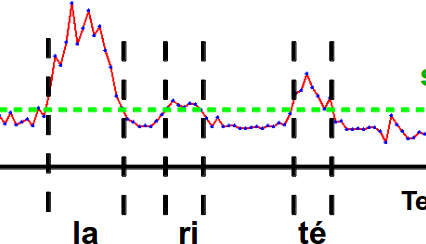
\includegraphics[width=\linewidth]{images/1.png}
\end{wrapfigure}

Ceci est un exercice de test. Il présente la syntaxe et les différentes fonctionnalités.

\question Première question de l'exercice. Faire ceci, faire cela.
\reponse{lkugf sqlkgdq us}
\subquestion Sous-question.
\question \subquestion Sousquestion
\reponse{$dqs\frac{1}{2} qd$}

\exercice{Exercice de test}

\begin{wrapfigure}{r}{.3\linewidth}
    \centering
    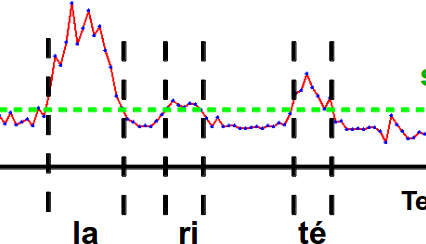
\includegraphics[width=\linewidth]{images/1.png}
\end{wrapfigure}

Ceci est un exercice de test. Il présente la syntaxe et les différentes fonctionnalités.

\question Première question de l'exercice. Faire ceci, faire cela.
\reponse{lkugf sqlkgdq us}
\subquestion Sous-question.
\question \subquestion Sousquestion
\reponse{$dqs\frac{1}{2} qd$}

\exercice{Exercice de test}

\begin{wrapfigure}{r}{.3\linewidth}
    \centering
    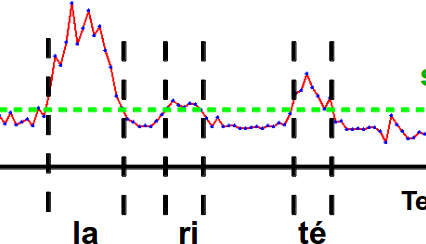
\includegraphics[width=\linewidth]{images/1.png}
\end{wrapfigure}

Ceci est un exercice de test. Il présente la syntaxe et les différentes fonctionnalités.

\question Première question de l'exercice. Faire ceci, faire cela.
\reponse{lkugf sqlkgdq us}
\subquestion Sous-question.
\question \subquestion Sousquestion
\reponse{$dqs\frac{1}{2} qd$}

\exercice{Exercice de test}

\begin{wrapfigure}{r}{.3\linewidth}
    \centering
    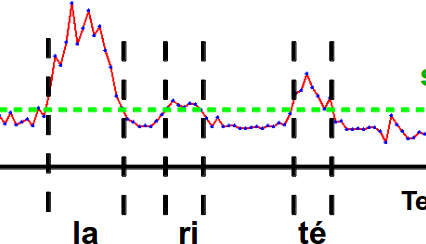
\includegraphics[width=\linewidth]{images/1.png}
\end{wrapfigure}

Ceci est un exercice de test. Il présente la syntaxe et les différentes fonctionnalités.

\question Première question de l'exercice. Faire ceci, faire cela.
\reponse{lkugf sqlkgdq us}
\subquestion Sous-question.
\question \subquestion Sousquestion
\reponse{$dqs\frac{1}{2} qd$}

\exercice{Exercice de test}

\begin{wrapfigure}{r}{.3\linewidth}
    \centering
    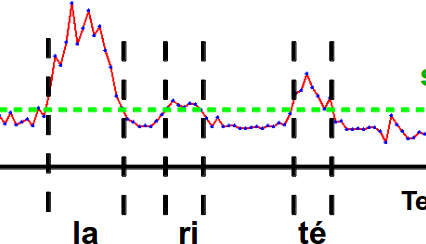
\includegraphics[width=\linewidth]{images/1.png}
\end{wrapfigure}

Ceci est un exercice de test. Il présente la syntaxe et les différentes fonctionnalités.

\question Première question de l'exercice. Faire ceci, faire cela.
\reponse{lkugf sqlkgdq us}
\subquestion Sous-question.
\question \subquestion Sousquestion
\reponse{$dqs\frac{1}{2} qd$}

\exercice{Exercice de test}

\begin{wrapfigure}{r}{.3\linewidth}
    \centering
    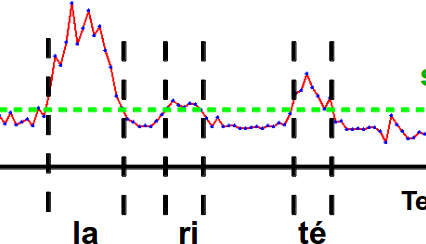
\includegraphics[width=\linewidth]{images/1.png}
\end{wrapfigure}

Ceci est un exercice de test. Il présente la syntaxe et les différentes fonctionnalités.

\question Première question de l'exercice. Faire ceci, faire cela.
\reponse{lkugf sqlkgdq us}
\subquestion Sous-question.
\question \subquestion Sousquestion
\reponse{$dqs\frac{1}{2} qd$}

